%==================================================================
\frame{\frametitle{Bipartite motifs} \label{back:motifList}

  \label{sec:motifList}
  \begin{tabular}{ll}
    \hspace{-.04\textwidth}
    \begin{tabular}{p{.45\textwidth}}
      \paragraph{'Meso-scale' analysis.} \refer{SCB19}
      \begin{itemize}
       \item Motifs ='building-blocks'
       \item between local (several nodes) and global (sub-graph)
      \end{itemize}
      \bigskip \bigskip 
      \paragraph{Interest.}
      \begin{itemize}
       \item Generic description of a network
       \item Enables network comparison
       \item Even when the nodes are different
      \end{itemize} \\
      \textcolor{gray}{($+$ 'species-role': out of the scope here)} \\
      \goto{sec:motifs}
    \end{tabular}
    &
    \begin{tabular}{p{.45\textwidth}} 
      \hspace{-0.035\textwidth}
      \includegraphics[width=.45\textwidth]{\fignet/SCB19-Oikos-Fig3-6motifs} \\      
    \end{tabular} 
  \end{tabular}

  \bigskip \bigskip 
  \paragraph{Existing tool.} \url{bmotif} package \refer{SSS19}: counts motif occurrences (\emphase{Not an easy task!})

}

%==================================================================
\frame{\frametitle{\BEDD model} \label{back:BEDD}

  \begin{tabular}{cccc}
    & & $h_0(v) =$ & $h(v) =$ \\
    \multicolumn{2}{c}{
      $\begin{array}{rl}
        \Pbb\{i \sim j \mid U_i, V_j\} & = \rho \; g(U_i) \; h(V_j) \\ \\
        \Esp (Y_{i+} \mid U_i) & = n \; \rho \; g(U_i) \\ \\
        \Esp (Y_{+j} \mid V_j) & = m \; \rho \; g(V_i) 
      \end{array}$
    } &
    \begin{tabular}{c} 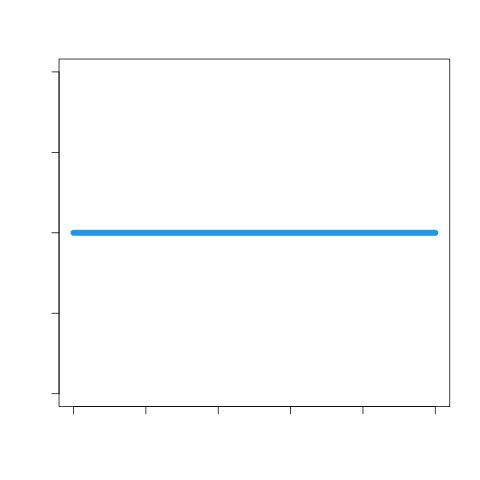
\includegraphics[width=.18\textwidth]{\fignet/FigMotifsBEDD-dist-h10} \end{tabular} &
    \begin{tabular}{c} 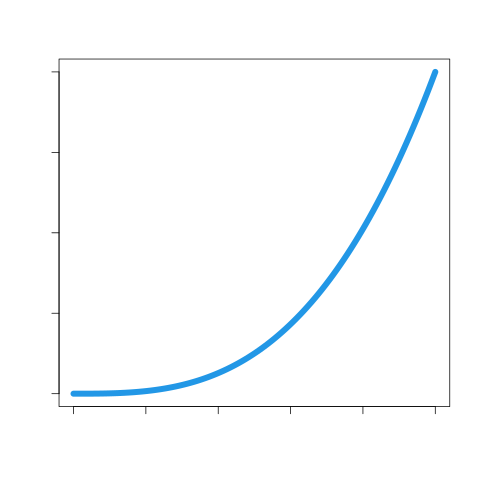
\includegraphics[width=.18\textwidth]{\fignet/FigMotifsBEDD-dist-h40} \end{tabular} \\
    \begin{tabular}{c} $g_0(u) =$ \end{tabular} &
    \begin{tabular}{c} 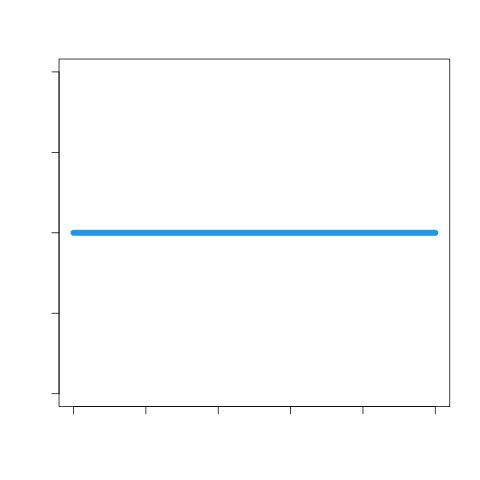
\includegraphics[width=.18\textwidth]{\fignet/FigMotifsBEDD-dist-g10} \end{tabular} &
    \begin{tabular}{c} 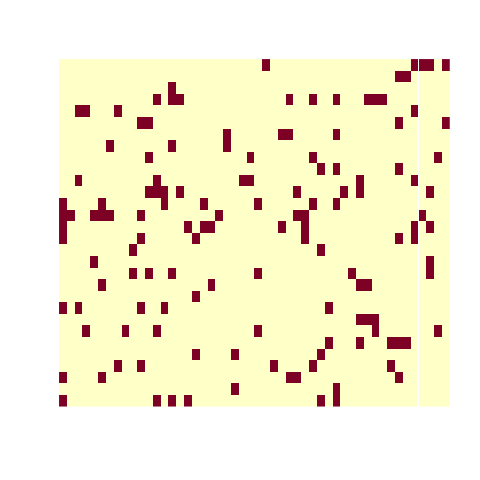
\includegraphics[width=.18\textwidth]{\fignet/FigMotifsBEDD-adj-g10-h10} \end{tabular} &
    \begin{tabular}{c} 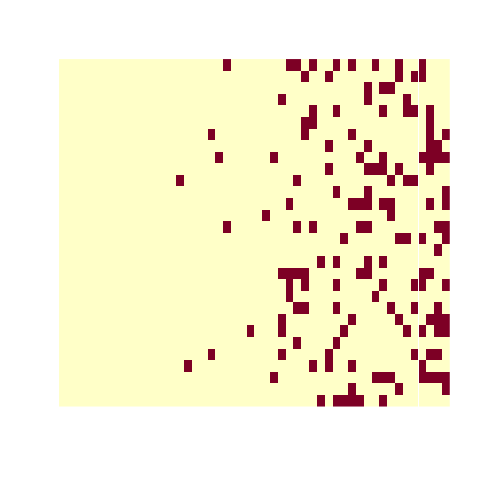
\includegraphics[width=.18\textwidth]{\fignet/FigMotifsBEDD-adj-g10-h40} \end{tabular} \\
    \begin{tabular}{c} $g(u) =$ \end{tabular} &
    \begin{tabular}{c} 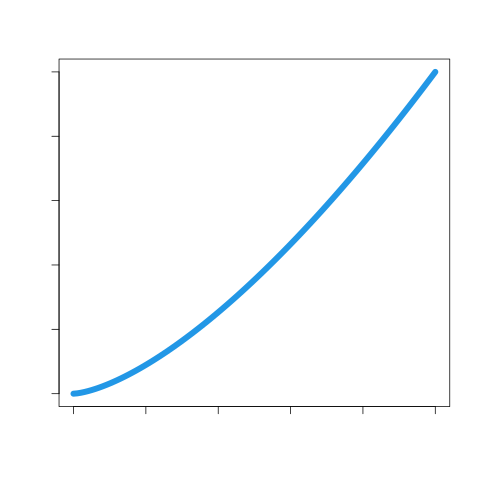
\includegraphics[width=.18\textwidth]{\fignet/FigMotifsBEDD-dist-g25} \end{tabular} &
    \begin{tabular}{c} 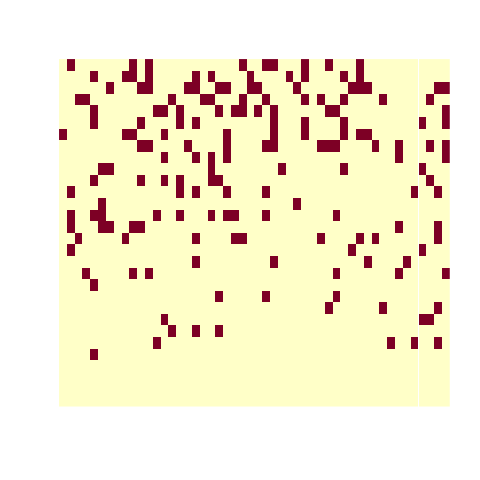
\includegraphics[width=.18\textwidth]{\fignet/FigMotifsBEDD-adj-g25-h10} \end{tabular} &
    \begin{tabular}{c} 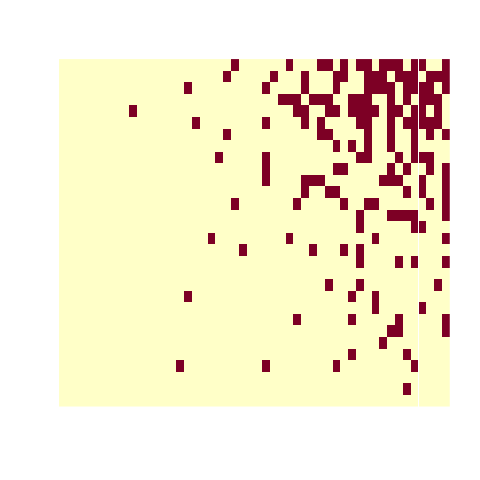
\includegraphics[width=.18\textwidth]{\fignet/FigMotifsBEDD-adj-g25-h40} \end{tabular} \\
  \end{tabular}
  
  \goto{sec:BEDD}
}

